%!LW recipe=uplatex

\documentclass[dvipdfmx]{standalone}

\usepackage{animate}
\usepackage{amsmath, amssymb, amsthm, mathrsfs, amsfonts, dsfont}
\usepackage{ascmac}
\usepackage{bbm}
\usepackage{bm}
\usepackage{breakcit
es}
\usepackage{calc}
\usepackage[style=base]{caption}
\usepackage{enumerate}
\usepackage[T1]{fontenc}
\usepackage{ifthen}
\usepackage{mathtools}
\usepackage{makecell}
\usepackage{mlmodern}
\usepackage{newtxtext}
\usepackage{optidef}
\usepackage[deluxe]{otf}
\usepackage{physics}
\usepackage{pifont}
\usepackage{setspace}
\usepackage{stfloats}
\usepackage{subcaption}
\usepackage{svg}
\usepackage{tikz}
\usepackage{xparse}
\usepackage[all]{xy}

\usepackage{float}
\usepackage{color}
\usepackage{graphicx}
\usepackage[colorlinks=true, allcolors=blue]{hyperref}


% === Commands ===

\definecolor{cA}{HTML}{0072BD}
\definecolor{cB}{HTML}{77AC30}
\definecolor{cC}{HTML}{0250b0}

\usetikzlibrary{
  3d,
  fit,
  calc,
  math,
  matrix,
  patterns,
  backgrounds,
  arrows.meta,
  decorations.pathmorphing,
}

\begin{document}

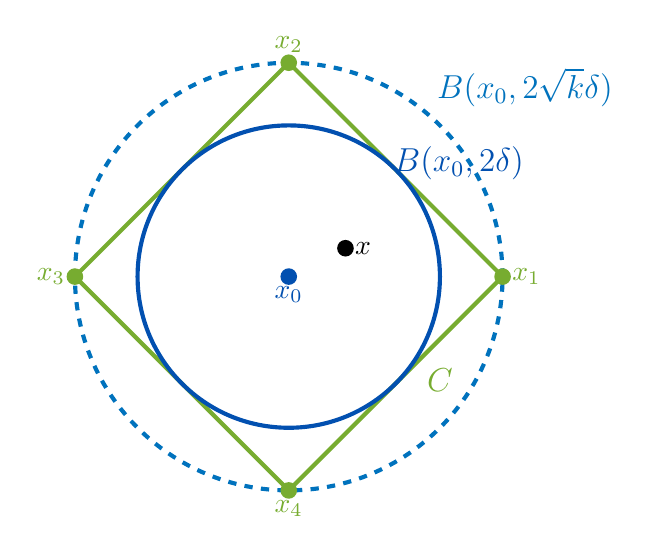
\begin{tikzpicture}[scale=1.2]

  % parameters
  \def\DELTA{0.8}
  \def\R{2*sqrt(2)*\DELTA}
  \def\r{2*\DELTA}

  % center
  \coordinate (x0) at (0,0);

  % vertices
  \coordinate (x1) at ({2*sqrt(2)*\DELTA},{0});
  \coordinate (x2) at ({0},{2*sqrt(2)*\DELTA});
  \coordinate (x3) at ({-2*sqrt(2)*\DELTA},{0});
  \coordinate (x4) at ({0},{-2*sqrt(2)*\DELTA});

  % outer ball B(x0,2sqrt2 delta)
  \draw[dashed,cA,line width=1.5pt] (x0) circle ({2*sqrt(2)*\DELTA});

  % square C = x0 + [-2δ,2δ]^2
  \draw[cB,line width=1.5pt] (x1) -- (x2) -- (x3) -- (x4) -- cycle;

  % inner ball B(x0,2δ)
  \draw[cC,line width=1.5pt] (x0) circle ({2*\DELTA});

  \fill[cB] (x1) circle (2.5pt) node[cB,right] {$x_1$};
  \fill[cB] (x2) circle (2.5pt) node[cB,above] {$x_2$};
  \fill[cB] (x3) circle (2.5pt) node[cB,left]  {$x_3$};
  \fill[cB] (x4) circle (2.5pt) node[cB,below] {$x_4$};

  % center point
  \fill[cC] (x0) circle (2.5pt) node[cC,below] {$x_0$};

  % sample point x in B(x0,2δ)
  \coordinate (x) at (0.6,0.3);
  \fill (x) circle (2.5pt) node[right] {$x$};

  % labels
  \node[cA,font=\large] at (2.5,2.0) {$B(x_0,2\sqrt{k}\delta)$};
  \node[cB,font=\large] at (1.6,-1.1)  {$C$};
  \node[cC,font=\large] at (1.8,1.2) {$B(x_0,2\delta)$};

\end{tikzpicture}

\end{document}
